\linespread{1.5}

O diagrama abaixo mostra uma seção esquemática do interior da Terra, onde destaca-se o manto terrestre, que se estende desde $r = 3480 km$ até $r = 6330$ km, sendo que a temperatura na base do manto é de $4000ºC$ e a temperatura no topo do manto é de $600ºC$.
\begin{figure}[H]
    \centering
    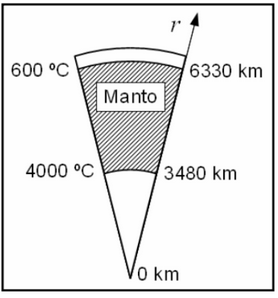
\includegraphics[width = 0.3\linewidth]{fig/edp16.png}
    \label{fig:edp16}
\end{figure}

Assumindo que a temperatura no interior terrestre seja radialmente simétrica (depende apenas do raio vetor e não depende das coordenadas angulares), pede-se:
\begin{itemize}
    \item[a)] Determine a função $u(r,t)$ que descreve a temperatura no interior do manto, sabendo que $u$ é solução estacionária (invariante no tempo) da equação de difusão de calor $u_t = a^2\nabla^2 u$, em coordenadas esféricas, sendo $a^2$ a difusividade térmica do manto; 
    \item[b)] Faça um esboço gráfico da temperatura no interior do manto;
    \item[c)] Calcule a temperatura no interior do manto, em $r=5000$ km.
\end{itemize}